\lecture{2}{2 May 2022}{}
\section[]{Calculus for Functions of \(\mathbb{R}^n\)}
We consider \(f \in C^2(\mathbb{R}^n)\), that is, all functions \(f: \mathbb{R}^n \to \mathbb{R}^n\) with continuous second derivatives. The point \(\mathbf{a} \in \mathbb{R}\) is \textit{stationary} if
\[
    \boldsymbol{\nabla}f(\mathbf{a}) = \eval{\partial_1 f, \dots, \partial_n f}_{\mathbf{x} = \mathbf{a}} = 0, \quad \partial_i f = \pd{f}{x^i}.
\]

If we expand near \(\mathbf{a}\), we have
\[
    f(\mathbf{x}) = f(\mathbf{a}) + (\mathbf{x} - \mathbf{a}) \cdot \eval{\boldsymbol{\nabla}}_{\mathbf{a}} + \frac{1}{2}(x_i - a_i)(x_j - a_j)\partial^2_{ij} \eval{f}_{\mathbf{a}} + \mathcal{O}(\abs{\mathbf{x} - \mathbf{a}}^2).
\]

The \textit{Hessian matrix} is \(H_{ij} = \partial_i \partial_j f = H_{ij}\). We shift the origin to set \(\mathbf{a} = \mathbf{0}\), and diagonalize \(H(\mathbf{0})\) by orthogonal transformation
\[
    H' = R^T H(\mathbf{0})R = \begin{psmallmatrix}
        \lambda_1 &  &  &   \\
         & \lambda_2 &  &   \\
         &  & \ddots &   \\
         &  &  &  \lambda_n \\
    \end{psmallmatrix}, \quad f(\mathbf{x}') - f(\mathbf{0}) = \frac{1}{2} \sum_i \lambda_i(x_i')^2 + \mathcal{O}(\abs{\mathbf{x}}^2).
\]
We consider several cases.
\begin{enumerate}
    \item If all \(\lambda_i > 0\), \(f(\mathbf{x}') > f(\mathbf{0})\) in all directions, it is a \textit{local minimum}.
    \item If all \(\lambda_i < 0\), \(f(\mathbf{x}') < f(\mathbf{0})\) in all directions, it is a \textit{local maximum}.
    \item If some \(\lambda_i > 0\) and some \(\lambda_i < 0\), \(f\) increases in some directions, and decreases in other directions. It is a \textit{saddle point}.
    \item If some \(\lambda_i = 0\) and the rest are of the same sign, we need to consider higher order terms in expansion.
\end{enumerate}
The special case when \(n = 2\), we have \(\det(H) = \lambda_1 \lambda_2\) and \(\tr(H) = \lambda_1 + \lambda_2\). If \(\det(H) > 0\), \(\tr(H) > 0\), it is a local minimum. If \(\det(H) < 0\), \(\tr(H) < 0\), it is a local maximum. If \(\det(H) < 0\), it is a saddle point. If \(\det(H) = 0\), we need to look at third and higher derivatives.

\begin{remark}
    \begin{enumerate}
        \item If \(f: D \to \mathbb{R}\) maps from a domain. We need to check boundary values too for global extrema.
        \item If \(f\) is harmonic on \(\mathbb{R}^2\), that is \(f_{xx} + f_{yy} = 0 \implies \tr(H) = 0\). If \(D \subsetneq \mathbb{R}^2\), all turning points are saddle points, and the extrema must be on the boundary.
    \end{enumerate}
\end{remark}
\begin{example}
    Take \(f(x, y) = x^3 + Y^3 - 3xy\), and we have \(\boldsymbol{\nabla}f = (3x^2 - 3y, 3y^2 - 3x)\). So the critical points are points where \(x^2 - y = 0\) and \(y^2 - x = 0\). So the stationary points are \(x = 0, y = 0\) and \(x = 1, y = 1\). The Hessian matrix is
    \[
        H = \begin{pmatrix}
            6x & -3 \\
            -3 & 6y \\
        \end{pmatrix}.
    \]
    At \((0,0)\), \(\det(H) = -9 < 0\), so it's a saddle point at \((0,0)\). And at \((1,1)\), \(\det(H) = 27 > 0\), \(\tr(H) = 12 > 0\), it is a local minimum.
    \begin{figure}[htpb]
        \centering
        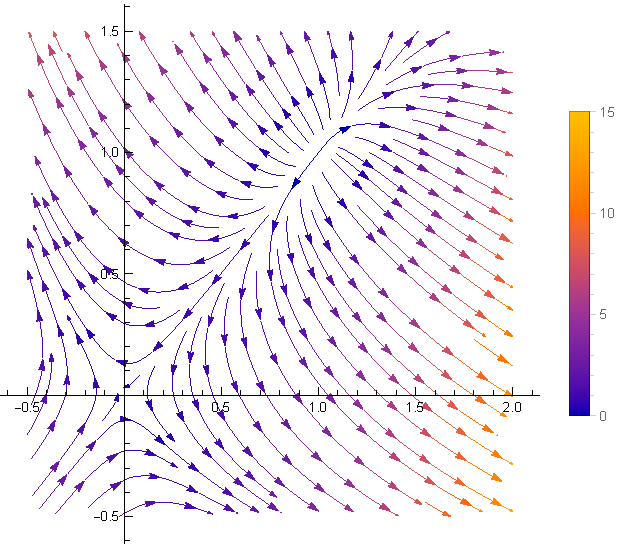
\includegraphics[width=0.5\textwidth]{Figures/fig_1_1.pdf}
        \caption{Plot of \(f\) showing the critical points}
        \label{fig_1_1}
    \end{figure}
\end{example}
\subsection{Constraints and Lagrange Multipliers}
\begin{example}
    Find the circle centered at \((0,0)\) with the smallest radius, which intersects the parabola \(y = x^2 - 1\).
    \begin{figure}[htpb]
        \centering
        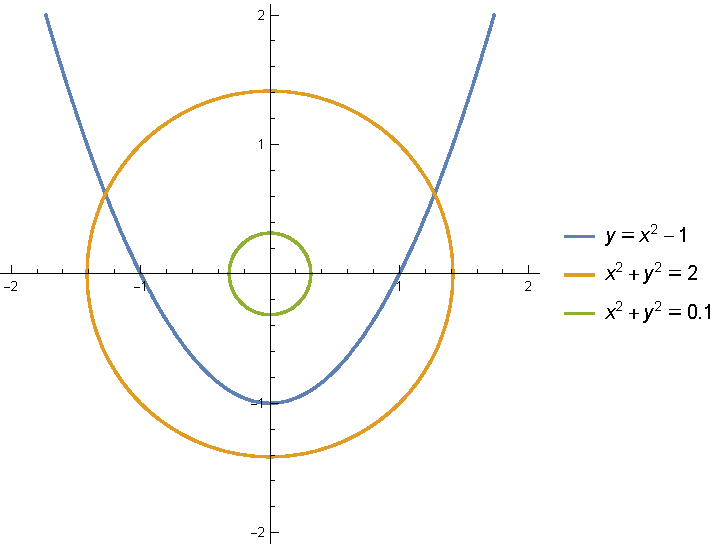
\includegraphics[width=0.5\textwidth]{Figures/fig_1_2.pdf}
        \caption{Circles and parabola}
        \label{fig_1_2}
    \end{figure}
    
    The direct method is to solve the constraints
    \[
        f = x^2 + y^2 = x^2 + (x^2 - 1)^2 = x^4 - x^2 + 1.
    \]
    If \(\partial f = 0\), we have \(4x^3 - 2x = 0\). So the solutions are \((0, -1)\) with radius \(1\) and \((\pm \frac{1}{\sqrt{2}}, -\frac{1}{2})\) with radius \(\frac{\sqrt{3}}{2} < 1\) which is the global minimum.

    The other method is \textit{Lagrange Multiplier}. Define \(h(x, y, \lambda) = f(x, y) - \lambda g(x, y)\) where \(g(x, y) = 0\) is the constraint and \(\lambda\) is the Lagrange multiplier. Now we extremize the function \(h(x,y) = x^2 + y^2 - \lambda(y - x^2 + 1)\)over 3 variables with no constraints; that is,
    \[
        \begin{dcases}
            \pd{h}{x} = 2x + 2\lambda x = 0\\
            \pd{h}{y} = 2y - \lambda = 0\\
            \pd{h}{\lambda} = y - x^2 + 1 = 0.
        \end{dcases}.
    \]
    Note that the last equation just gives the constraint back. The solutions are \((0, -1)\) and \((\pm \frac{1}{\sqrt{2}}, -\frac{1}{2})\) as before will \(\lambda = -2\) and \(\lambda = -1\), respectively.
\end{example}

We show that Lagrange Multiplier works by geometry.
\begin{figure}[htpb]
    \centering
    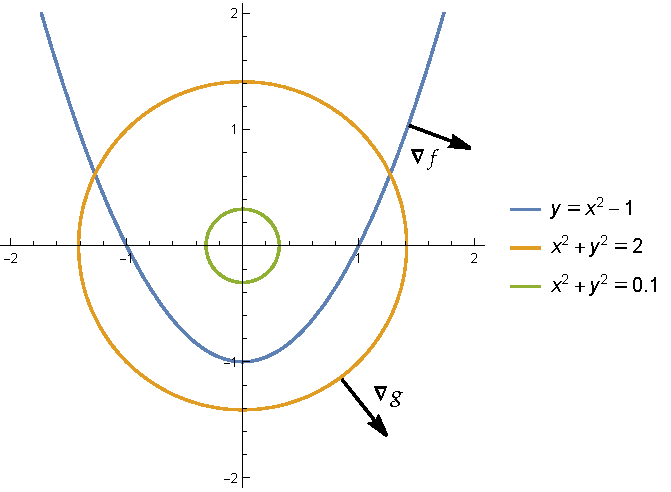
\includegraphics[width=0.5\textwidth]{Figures/fig_1_3.pdf}
    \caption{Gradients of the functions}
    \label{fig:fig_1_3}
\end{figure}

We know that \(\boldsymbol{\nabla}g\) is perpendicular to \(g = 0\) and \(\boldsymbol{\nabla}f\) is perpendicular to \(f\) being constant. They must be parallel so \(\boldsymbol{\nabla}f = \lambda \boldsymbol{\nabla} g\) and \(\boldsymbol{\nabla}(f - \lambda g) = 0\).

If we have multiple constraints with \(f: \mathbb{R}^n \to \mathbb{R}\) subject to \(g_a(\mathbf{x}) = 0\) for \(a = 1, \dots, k\), then we let
\[
    h(x_1, \dots, x_n, \lambda_1, \dots, \lambda_k) = f - \sum_a \lambda_a g_a.
\]
And solve for \(\pd{h}{x^i} = 0\) and \(\pd{h}{\lambda^i} = 0\).
